\documentclass[11pt,a4paper,]{article}
\usepackage{lmodern}

\usepackage{amssymb,amsmath}
\usepackage{ifxetex,ifluatex}
\usepackage{fixltx2e} % provides \textsubscript
\ifnum 0\ifxetex 1\fi\ifluatex 1\fi=0 % if pdftex
  \usepackage[T1]{fontenc}
  \usepackage[utf8]{inputenc}
\else % if luatex or xelatex
  \usepackage{unicode-math}
  \defaultfontfeatures{Ligatures=TeX,Scale=MatchLowercase}
\fi
% use upquote if available, for straight quotes in verbatim environments
\IfFileExists{upquote.sty}{\usepackage{upquote}}{}
% use microtype if available
\IfFileExists{microtype.sty}{%
\usepackage[]{microtype}
\UseMicrotypeSet[protrusion]{basicmath} % disable protrusion for tt fonts
}{}
\PassOptionsToPackage{hyphens}{url} % url is loaded by hyperref
\usepackage[unicode=true]{hyperref}
\hypersetup{
            pdftitle={ETC5513 Assignment 4},
            pdfborder={0 0 0},
            breaklinks=true}
\urlstyle{same}  % don't use monospace font for urls
\usepackage{geometry}
\geometry{a4paper, centering, text={16cm,24cm}}
\usepackage[style=authoryear-comp,]{biblatex}
\addbibresource{references.bib}
\usepackage{longtable,booktabs}
% Fix footnotes in tables (requires footnote package)
\IfFileExists{footnote.sty}{\usepackage{footnote}\makesavenoteenv{long table}}{}
\usepackage{graphicx,grffile}
\makeatletter
\def\maxwidth{\ifdim\Gin@nat@width>\linewidth\linewidth\else\Gin@nat@width\fi}
\def\maxheight{\ifdim\Gin@nat@height>\textheight\textheight\else\Gin@nat@height\fi}
\makeatother
% Scale images if necessary, so that they will not overflow the page
% margins by default, and it is still possible to overwrite the defaults
% using explicit options in \includegraphics[width, height, ...]{}
\setkeys{Gin}{width=\maxwidth,height=\maxheight,keepaspectratio}
\IfFileExists{parskip.sty}{%
\usepackage{parskip}
}{% else
\setlength{\parindent}{0pt}
\setlength{\parskip}{6pt plus 2pt minus 1pt}
}
\setlength{\emergencystretch}{3em}  % prevent overfull lines
\providecommand{\tightlist}{%
  \setlength{\itemsep}{0pt}\setlength{\parskip}{0pt}}
\setcounter{secnumdepth}{5}

% set default figure placement to htbp
\makeatletter
\def\fps@figure{htbp}
\makeatother


\title{ETC5513 Assignment 4}

%% MONASH STUFF

%% CAPTIONS
\RequirePackage{caption}
\DeclareCaptionStyle{italic}[justification=centering]
 {labelfont={bf},textfont={it},labelsep=colon}
\captionsetup[figure]{style=italic,format=hang,singlelinecheck=true}
\captionsetup[table]{style=italic,format=hang,singlelinecheck=true}


%% FONT
\RequirePackage{bera}
\RequirePackage[charter,expert,sfscaled]{mathdesign}
\RequirePackage{fontawesome}

%% HEADERS AND FOOTERS
\RequirePackage{fancyhdr}
\pagestyle{fancy}
\rfoot{\Large\sffamily\raisebox{-0.1cm}{\textbf{\thepage}}}
\makeatletter
\lhead{\textsf{\expandafter{\@title}}}
\makeatother
\rhead{}
\cfoot{}
\setlength{\headheight}{15pt}
\renewcommand{\headrulewidth}{0.4pt}
\renewcommand{\footrulewidth}{0.4pt}
\fancypagestyle{plain}{%
\fancyhf{} % clear all header and footer fields
\fancyfoot[C]{\sffamily\thepage} % except the center
\renewcommand{\headrulewidth}{0pt}
\renewcommand{\footrulewidth}{0pt}}

%% MATHS
\RequirePackage{bm,amsmath}
\allowdisplaybreaks

%% GRAPHICS
\RequirePackage{graphicx}
\setcounter{topnumber}{2}
\setcounter{bottomnumber}{2}
\setcounter{totalnumber}{4}
\renewcommand{\topfraction}{0.85}
\renewcommand{\bottomfraction}{0.85}
\renewcommand{\textfraction}{0.15}
\renewcommand{\floatpagefraction}{0.8}


%\RequirePackage[section]{placeins}

%% SECTION TITLES


%% SECTION TITLES (NEW: Changing sections and subsections color)
\RequirePackage[compact,sf,bf]{titlesec}
\titleformat*{\section}{\Large\sf\bfseries\color[rgb]{0.8, 0.7, 0.1 }}
\titleformat*{\subsection}{\large\sf\bfseries\color[rgb]{0.8, 0.7, 0.1 }}
\titleformat*{\subsubsection}{\sf\bfseries\color[rgb]{0.8, 0.7, 0.1 }}
\titlespacing{\section}{0pt}{2ex}{.5ex}
\titlespacing{\subsection}{0pt}{1.5ex}{0ex}
\titlespacing{\subsubsection}{0pt}{.5ex}{0ex}


%% TITLE PAGE
\def\Date{\number\day}
\def\Month{\ifcase\month\or
 January\or February\or March\or April\or May\or June\or
 July\or August\or September\or October\or November\or December\fi}
\def\Year{\number\year}

%% LINE AND PAGE BREAKING
\sloppy
\clubpenalty = 10000
\widowpenalty = 10000
\brokenpenalty = 10000
\RequirePackage{microtype}

%% PARAGRAPH BREAKS
\setlength{\parskip}{1.4ex}
\setlength{\parindent}{0em}

%% HYPERLINKS
\RequirePackage{xcolor} % Needed for links
\definecolor{darkblue}{rgb}{0,0,.6}
\RequirePackage{url}

\makeatletter
\@ifpackageloaded{hyperref}{}{\RequirePackage{hyperref}}
\makeatother
\hypersetup{
     citecolor=0 0 0,
     breaklinks=true,
     bookmarksopen=true,
     bookmarksnumbered=true,
     linkcolor=darkblue,
     urlcolor=blue,
     citecolor=darkblue,
     colorlinks=true}

\usepackage[showonlyrefs]{mathtools}
\usepackage[no-weekday]{eukdate}

%% BIBLIOGRAPHY

\makeatletter
\@ifpackageloaded{biblatex}{}{\usepackage[style=authoryear-comp, backend=biber, natbib=true]{biblatex}}
\makeatother
\ExecuteBibliographyOptions{bibencoding=utf8,minnames=1,maxnames=3, maxbibnames=99,dashed=false,terseinits=true,giveninits=true,uniquename=false,uniquelist=false,doi=false, isbn=false,url=true,sortcites=false}

\DeclareFieldFormat{url}{\texttt{\url{#1}}}
\DeclareFieldFormat[article]{pages}{#1}
\DeclareFieldFormat[inproceedings]{pages}{\lowercase{pp.}#1}
\DeclareFieldFormat[incollection]{pages}{\lowercase{pp.}#1}
\DeclareFieldFormat[article]{volume}{\mkbibbold{#1}}
\DeclareFieldFormat[article]{number}{\mkbibparens{#1}}
\DeclareFieldFormat[article]{title}{\MakeCapital{#1}}
\DeclareFieldFormat[article]{url}{}
%\DeclareFieldFormat[book]{url}{}
%\DeclareFieldFormat[inbook]{url}{}
%\DeclareFieldFormat[incollection]{url}{}
%\DeclareFieldFormat[inproceedings]{url}{}
\DeclareFieldFormat[inproceedings]{title}{#1}
\DeclareFieldFormat{shorthandwidth}{#1}
%\DeclareFieldFormat{extrayear}{}
% No dot before number of articles
\usepackage{xpatch}
\xpatchbibmacro{volume+number+eid}{\setunit*{\adddot}}{}{}{}
% Remove In: for an article.
\renewbibmacro{in:}{%
  \ifentrytype{article}{}{%
  \printtext{\bibstring{in}\intitlepunct}}}

\AtEveryBibitem{\clearfield{month}}
\AtEveryCitekey{\clearfield{month}}

\makeatletter
\DeclareDelimFormat[cbx@textcite]{nameyeardelim}{\addspace}
\makeatother

\author{\sf\Large\textbf{ Yiwen Jiang}\\ {\sf\large BComm\\[0.5cm]} \sf\Large\textbf{ Helen Evangelina}\\ {\sf\large BComm\\[0.5cm]} \sf\Large\textbf{ Ruimin Lin}\\ {\sf\large BComm\\[0.5cm]} \sf\Large\textbf{ XXX XXX}\\ {\sf\large XXX\\[0.5cm]}}

\date{\sf\Date~\Month~\Year}
\makeatletter
\lfoot{\sf Jiang, Evangelina, Lin, XXX: \@date}
\makeatother


%%%% PAGE STYLE FOR FRONT PAGE OF REPORTS

\makeatletter
\def\organization#1{\gdef\@organization{#1}}
\def\telephone#1{\gdef\@telephone{#1}}
\def\email#1{\gdef\@email{#1}}
\makeatother
  \organization{Australian Bureau of Statistic}

  \def\name{Our consultancy \newline add names \&\newline add names}

  \telephone{(03) 9905 2478}

  \email{questions@company.com}                 %NEW: New email addresss

\def\webaddress{\url{http://company.com/stats/consulting/}} %NEW: URl
\def\abn{12 377 614 630}                                    % NEW: ABN
\def\logo{\includegraphics[width=6cm]{logo}}  %NEW: Changing logo
\def\extraspace{\vspace*{1.6cm}}
\makeatletter
\def\contactdetails{\faicon{phone} & \@telephone \\
                    \faicon{envelope} & \@email}
\makeatother

%%%% FRONT PAGE OF REPORTS

\def\reporttype{Report for}

\long\def\front#1#2#3{
\newpage
\begin{singlespacing}
\thispagestyle{empty}
\vspace*{-1.4cm}
\hspace*{-1.4cm}
\hbox to 16cm{
  \hbox to 6.5cm{\vbox to 14cm{\vbox to 25cm{
    \logo
    \vfill
    \parbox{6.3cm}{\raggedright
      \sf\color[rgb]{0.8, 0.7, 0.1 }    % NEW color 
      {\large\textbf{\name}}\par
      \vspace{.7cm}
      \tabcolsep=0.12cm\sf\small
      \begin{tabular}{@{}ll@{}}\contactdetails
      \end{tabular}
      \vspace*{0.3cm}\par
      ABN: \abn\par
    }
  }\vss}\hss}
  \hspace*{0.2cm}
  \hbox to 1cm{\vbox to 14cm{\rule{4pt}{26.8cm}\vss}\hss\hfill}  %NEW: Thicker line
  \hbox to 10cm{\vbox to 14cm{\vbox to 25cm{   
      \vspace*{3cm}\sf\raggedright
      \parbox{11cm}{\sf\raggedright\baselineskip=1.2cm
         \fontsize{24.88}{30}\color[rgb]{0, 0.29, 0.55}\sf\textbf{#1}}   % NEW: title color blue
      \par
      \vfill
      \large
      \vbox{\parskip=0.8cm #2}\par
      \vspace*{2cm}\par
      \reporttype\\[0.3cm]
      \hbox{#3}%\\[2cm]\
      \vspace*{1cm}
      {\large\sf\textbf{\Date~\Month~\Year}}
   }\vss}
  }}
\end{singlespacing}
\newpage
}

\makeatletter
\def\titlepage{\front{\expandafter{\@title}}{\@author}{\@organization}}
\makeatother

\usepackage{setspace}
\setstretch{1.5}

%% Any special functions or other packages can be loaded here.
\usepackage{float}
\let\origfigure\figure
\let\endorigfigure\endfigure
\renewenvironment{figure}[1][2] {
\expandafter\origfigure\expandafter[H]
} {
\endorigfigure
}
\usepackage{booktabs}
\usepackage{longtable}
\usepackage{array}
\usepackage{multirow}
\usepackage{wrapfig}
\usepackage{float}
\usepackage{colortbl}
\usepackage{pdflscape}
\usepackage{tabu}
\usepackage{threeparttable}
\usepackage{threeparttablex}
\usepackage[normalem]{ulem}
\usepackage{makecell}
\usepackage{xcolor}


\begin{document}
\titlepage

{
\setcounter{tocdepth}{2}
\tableofcontents
}
\newpage

\hypertarget{introduction}{%
\section{Introduction}\label{introduction}}

The number and rate of offences in Australia are affected by various factors. In recent year, Australia is continually strengthening law enforcement. Although this can reduce the offence rate, the number of offences is also rising with the continuous increase of the population. This report shows the current status of criminal activity in Australia and changes in criminal activity in terms of age, gender, states or territories, and police proceeding.

In the first section, look at the offenders by age group in Australia. The purpose is to explore the distribution of offenders across age groups, what principal offences account for the majority of the offences in each age group, and the changes in the number of offenders by year. By conducting this analysis, an overview of the distribution and trend of the number of offenders by age group can be obtained.

Although the status of female offence in modern society is more prominent than in the past, it is a recognised fact that in general, under various social systems and historical conditions, the proportion of female offenders in the total number of offenders is significantly lower. At the same time, the gender difference in the number of offences has more significant uncertainty. We will analyse the number and rate of offenders for each gender and explore the yearly changes of the offences on each gender group in the second section.

For section three, we analyse the crime statistics on states or territories in Australia. The intention is to explore how the primary offences take account in each state or territory in 2018, and which state or territory have competitively higher crime rates. By analysing the crime statistics on states or territories, the report will offer insights on how each state or territory differs on the frequency of primary offences recorded.

Furthermore, in the fourth section, we analyse the court actions of offenders in Australia. The purpose of this section is to investigate the distribution of court and non-court actions of offenders in each state, and which specific crime will be resulting in more court actions than non-court actions. By analyse the court actions of the criminal, we also provide some detailed explanations and the possible reason to cause this phenomenon.

\newpage

\hypertarget{analysis}{%
\section{Analysis}\label{analysis}}

\section*{Gender difference in the number and rate of offences}

\begin{verbatim}
## `summarise()` regrouping output by 'year', 'offence_type' (override with `.groups` argument)
\end{verbatim}

\begin{figure}
\centering
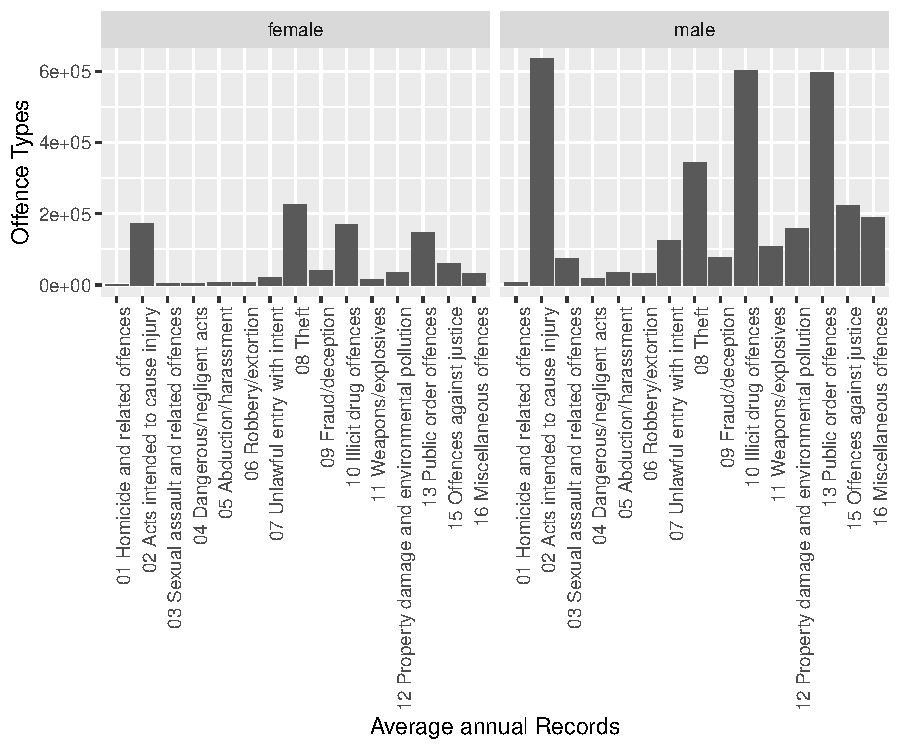
\includegraphics{ETC5513-Assignment4_files/figure-latex/gender1-1.pdf}
\caption{\label{fig:gender1}Yearly average offence records of different offence type}
\end{figure}

As showing in Figure \ref{fig:gender1}, each bar represents the average number of records for each type of offence and gender over the ten years. The overall offence recorded that the number of male offenders is significantly higher than female offenders. The highest number of offence type for males are ``Acts intended to cause injury'' and for females are ``Theft''.

\begin{verbatim}
## `summarise()` ungrouping output (override with `.groups` argument)
\end{verbatim}

If we look at the summary (Refer to Table \ref{tab:gendersumm}), the result also indicates that in all the offence types, the number of male offenders is significantly higher than female offenders. The ``Sexual assault and related offence'' is the most significant difference between the number of males and females, and the average number of males is about 17 times higher than females. The difference in ``Theft'' is relatively minimal; males are about 1.53 times higher than females. Over the ten years, the average number of male offenders is 4.42 times higher than that of females.

\begin{figure}
\centering
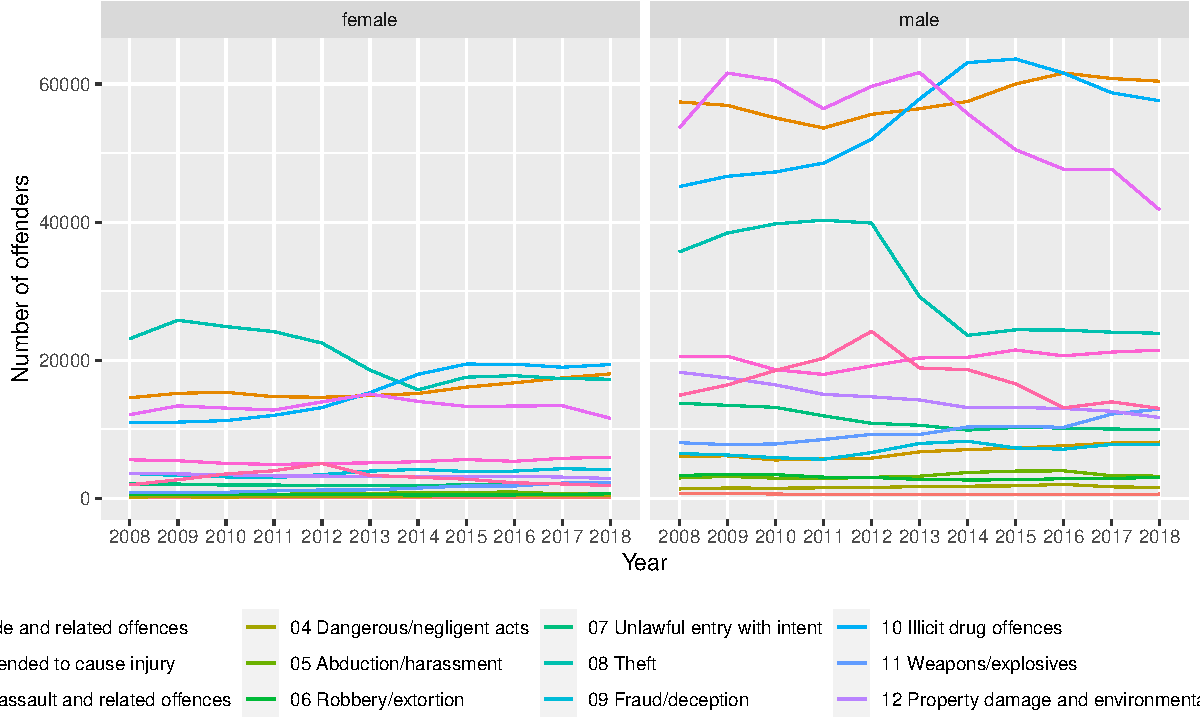
\includegraphics{ETC5513-Assignment4_files/figure-latex/gender2-1.pdf}
\caption{\label{fig:gender2}Yearly Number of Offenders on Female and Male}
\end{figure}

From Figure \ref{fig:gender2}, we can observe that the yearly changes on the number of records of most types of the offence are stable on both genders. However, there still have some changes. For females, the number of ``Theft'' drop highly, from about 25,000 reduced to 15,000 and ``Illicit drug offences'' increased by nearly 10,000. For males, although some type offences remain at a relatively high level, ``Unlawful entry with intent and Property damage'' and ``environmental pollution'' have decreased by about 20,000. Government still need to pay attention to the issue of ``Illicit drug offences'', because the number of records has increased a lot compared to 2008.

\begin{figure}
\centering
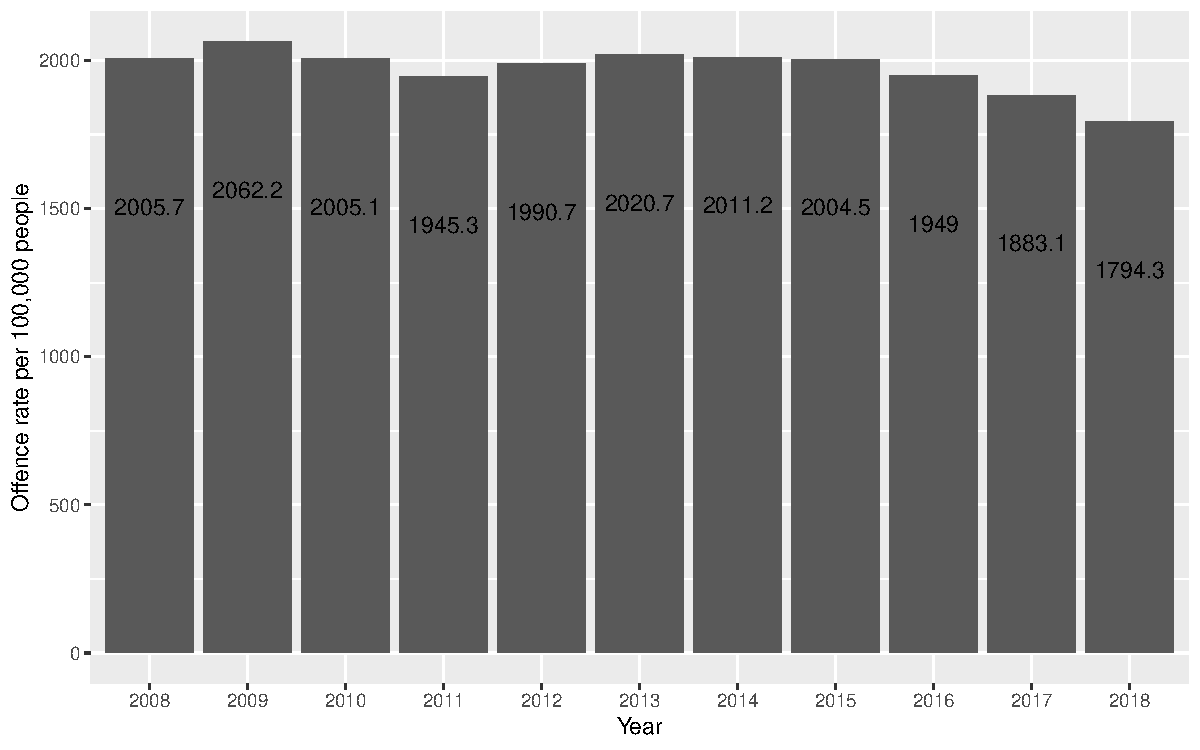
\includegraphics{ETC5513-Assignment4_files/figure-latex/gender3-1.pdf}
\caption{\label{fig:gender3}Rate of offenders recorded in Australia}
\end{figure}

In Figure \ref{fig:gender3}, it represents the offender rate on both genders; the rate indicates the number of offenders in 100,000 people. In 2009, the rate was 2,062 offenders in 100,000 people. After the overall trend is decreasing, in 2018, there are about 1,794 offenders in 100,000 people. The rate decreased to their lowest levels in six years.

Focus on the change on the genders (Refer to Table \ref{tab:gendersumm2}); the rate of both genders offenders is continuously decreasing in recent years.

From Table \ref{tab:gendersumm3}, we can conclude that the number of offenders recorded in Australia increased on both males and females from 2008 to 2018. However, the rate of offenders recorded has dropped significantly, and the offence rate of males has decreased more than that of females.

\begin{itemize}
\tightlist
\item
  The number of male offenders increased by 5,239, and the increasing rate is 1.79\%.\\
\item
  The number of female offenders increased by 13,595, and the increasing rate is 16.63\%.\\
\item
  The rate of male offenders has dropped by 408 per 100,000 people, and the decreasing rate is 12.93\%.\\
\item
  The rate of female offenders has dropped by 9 per 100,000 people, and the decreasing rate is 1.07\%.
\end{itemize}

\pagebreak

\section*{Crime analysis by age group}

\begin{verbatim}
## `summarise()` ungrouping output (override with `.groups` argument)
\end{verbatim}

\begin{figure}
\centering
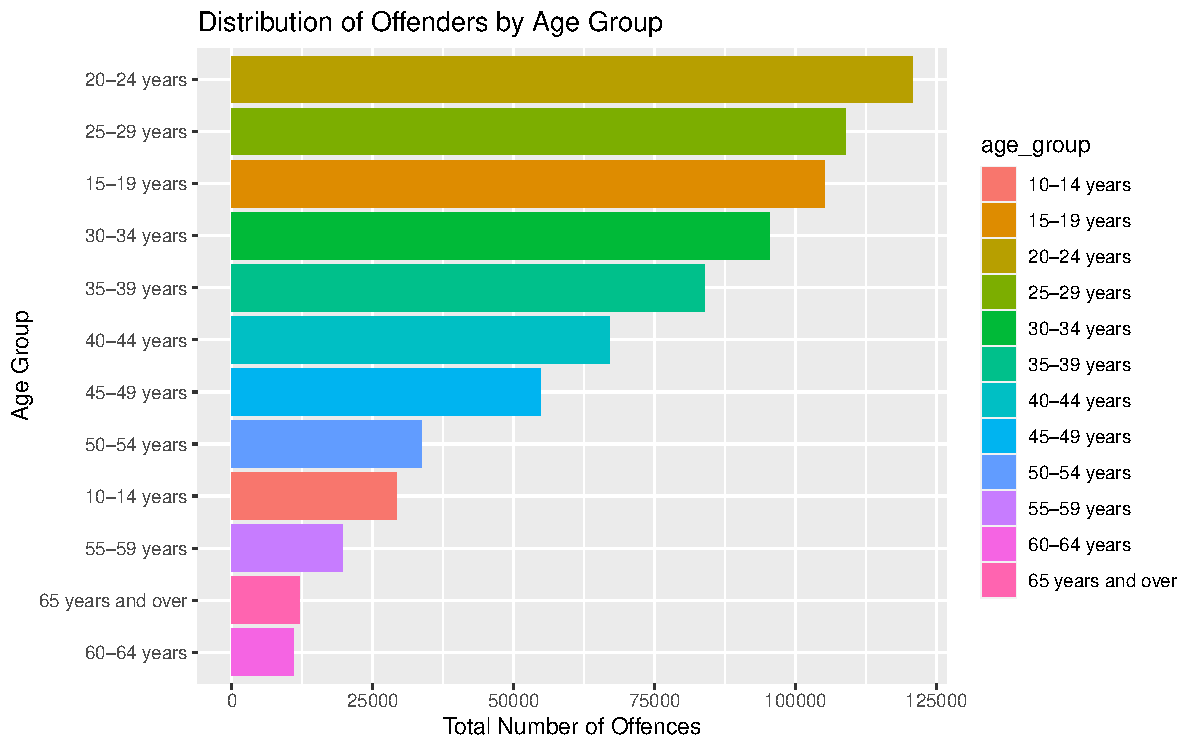
\includegraphics{ETC5513-Assignment4_files/figure-latex/age1-1.pdf}
\caption{\label{fig:age1}Total offenders across age groups}
\end{figure}

Figure \ref{fig:age1} shows the distribution of offenders across age groups, with each bar representing the total number of offences for certain age group. The highest proportion of offenders is from the age of 20-24 years, followed by 25-29 and 15-19 years, while the lowest proportion of offenders is from 60-64 years age group. This indicates that older people tend to not commit an offence and the majority of offenders are young people.

\begin{verbatim}
## `summarise()` regrouping output by 'age_group' (override with `.groups` argument)
\end{verbatim}

\begin{figure}
\centering
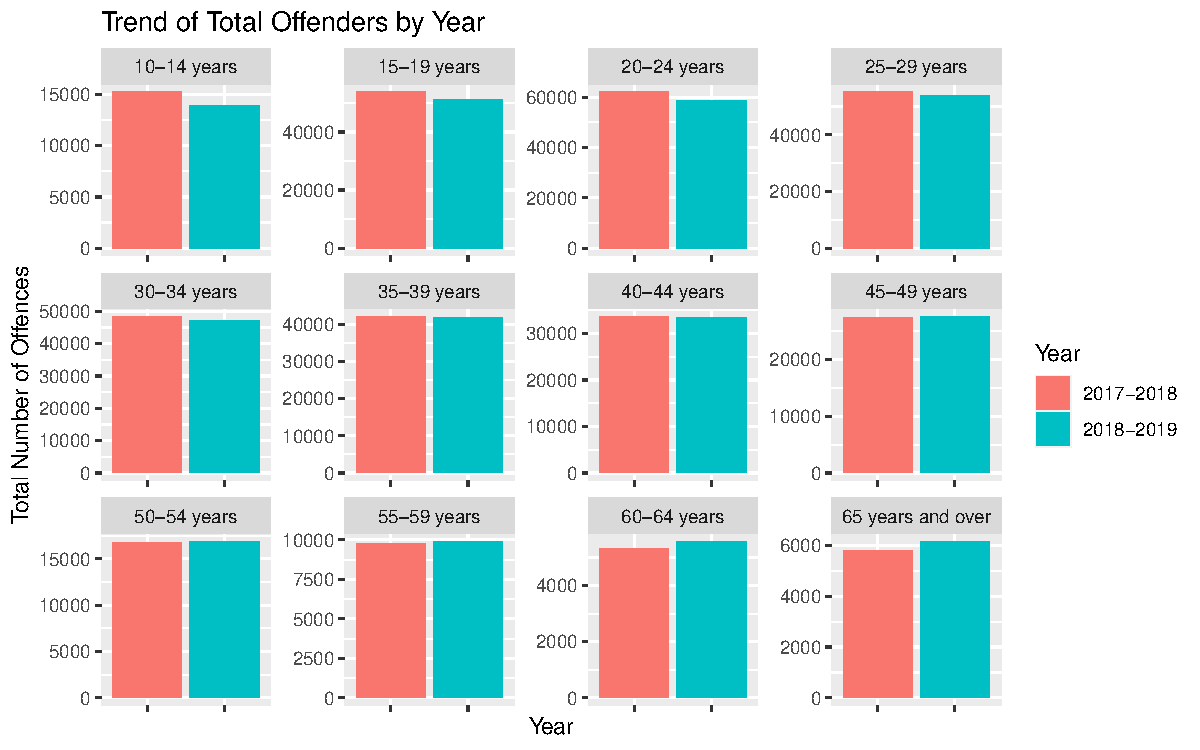
\includegraphics{ETC5513-Assignment4_files/figure-latex/age-yearly-changes-1.pdf}
\caption{\label{fig:age-yearly-changes}Distribution of total offenders yearly}
\end{figure}

\begin{verbatim}
## `summarise()` ungrouping output (override with `.groups` argument)
## `summarise()` ungrouping output (override with `.groups` argument)
\end{verbatim}

An interesting trend to notice from Figure \ref{fig:age-yearly-changes} and Table \ref{tab:summary-table} is that the number of offences for age group below 45 decreased in 2018-2019, while it increased for age group above 45. This is due to the structural ageing that is experienced by all Australian states and territories (\textcite{AIC}). The overall changes however are not that high. Age group 10-14 years has the most significant change which is a decrease of 1310 or around -8.6\%. And the age group with the least change is 35-39 years which is only a decrease of 68. The number of offences commited by middle age groups do not change much.

Next, we are looking at the top three highest and lowest age group in more details.

\begin{verbatim}
## `summarise()` regrouping output by 'age_group', 'principal_offence' (override with `.groups` argument)
\end{verbatim}

\begin{figure}
\centering
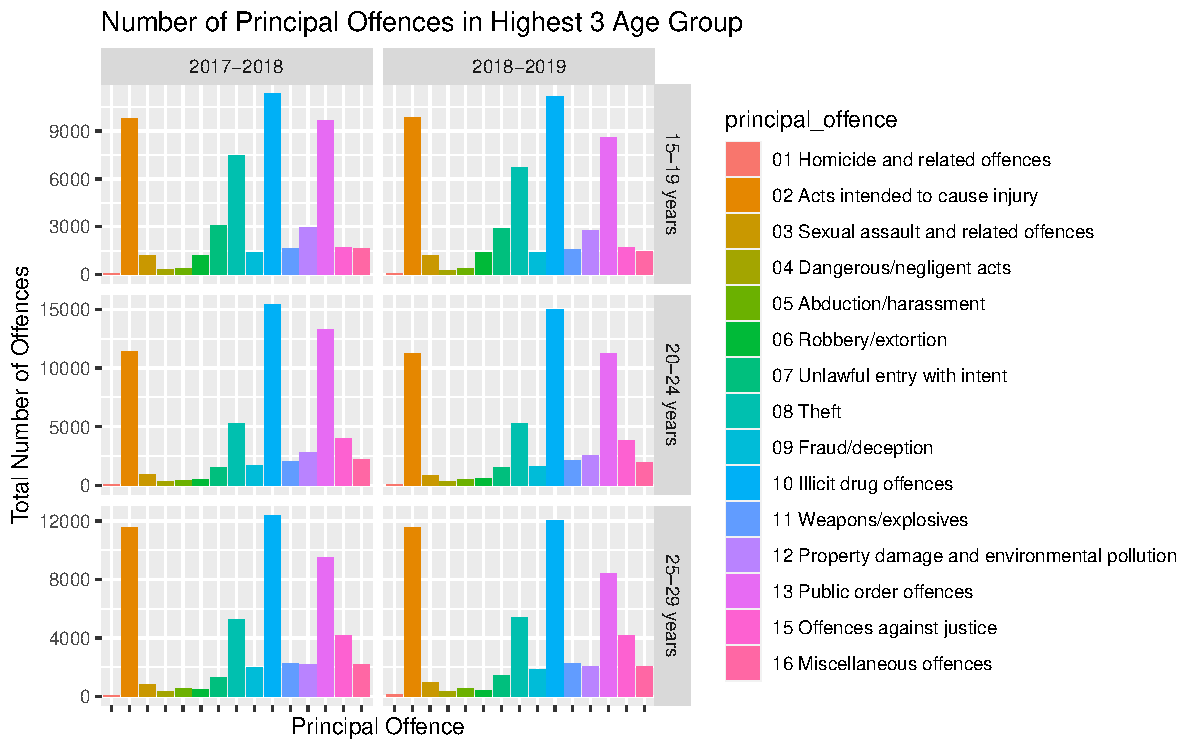
\includegraphics{ETC5513-Assignment4_files/figure-latex/topage-1.pdf}
\caption{\label{fig:topage}Top three highest age group principal offences}
\end{figure}

From Figure \ref{fig:topage}, we can see a clear trend here that all age group has the highest number of offences in illicit drug offences. However, the number is decreasing in 2018-2019, which is resulted from `lower level' offences being diverted from the courts (\textcite{AIHW}). While the changes in other types of offence seem to be little, the changes for ``Public order offences'' seems to be high.

\begin{verbatim}
## `summarise()` regrouping output by 'age_group', 'principal_offence' (override with `.groups` argument)
\end{verbatim}

\begin{figure}
\centering
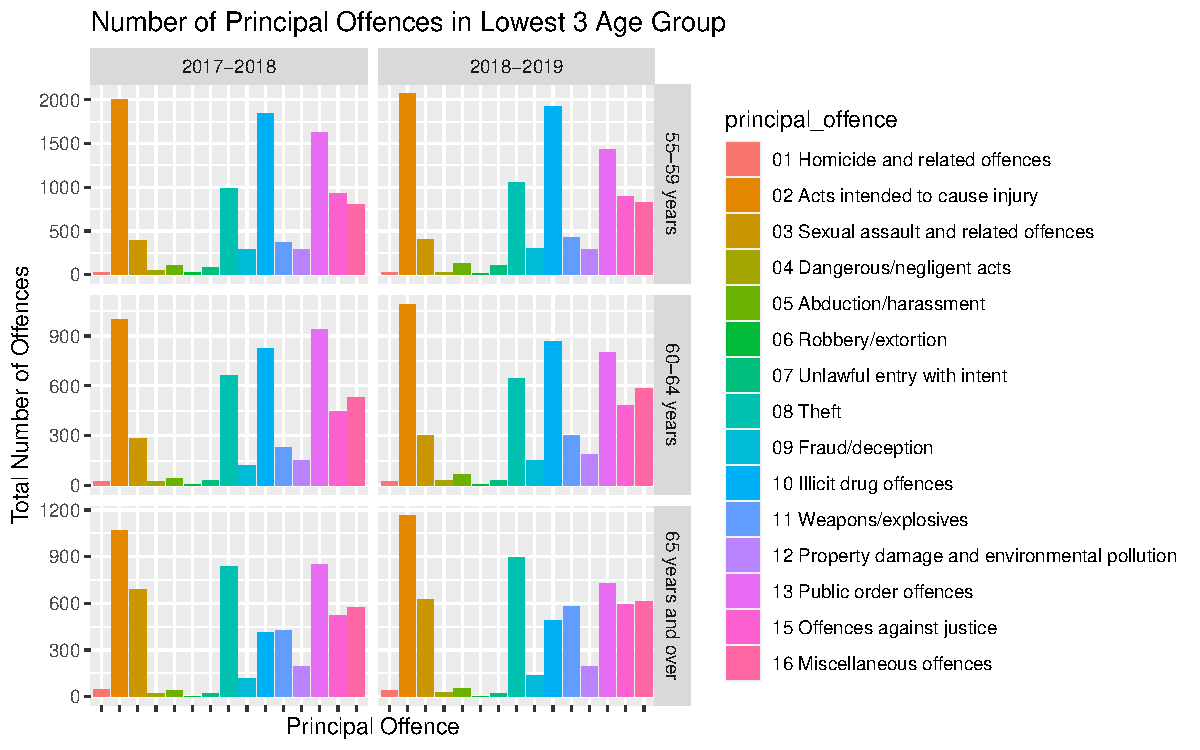
\includegraphics{ETC5513-Assignment4_files/figure-latex/lowestage-1.pdf}
\caption{\label{fig:lowestage}Lowest three highest age group principal offences}
\end{figure}

Figure \ref{fig:lowestage} illustrates the distribution of total offenders in each principal offences for the lowest 3 age groups. There are some differences compared to the top 3 age groups. The highest principal offence for these lowest 3 groups is ``Acts intended to cause injury''. Interesting findings here are that total offenders in ``Illicit drug offences'' decreased as the age group moves up and also ``Offences against justice'' and ``Miscellaneous offences'' tend to be higher in older ages compared to younger ages. While most of the offence types experienced an increase over time, one similar finding as in the top 3 data is that there is a significant decrease in ``Public order offences''.

\pagebreak

\section*{Crime analysis by State and Territory}

In this section, we are exploring the Australian crime statistics between states/territories. The analysis will be exploring which state has the highest crime rates, and what principal offence accounts for a large proportion.

\begin{figure}
\centering
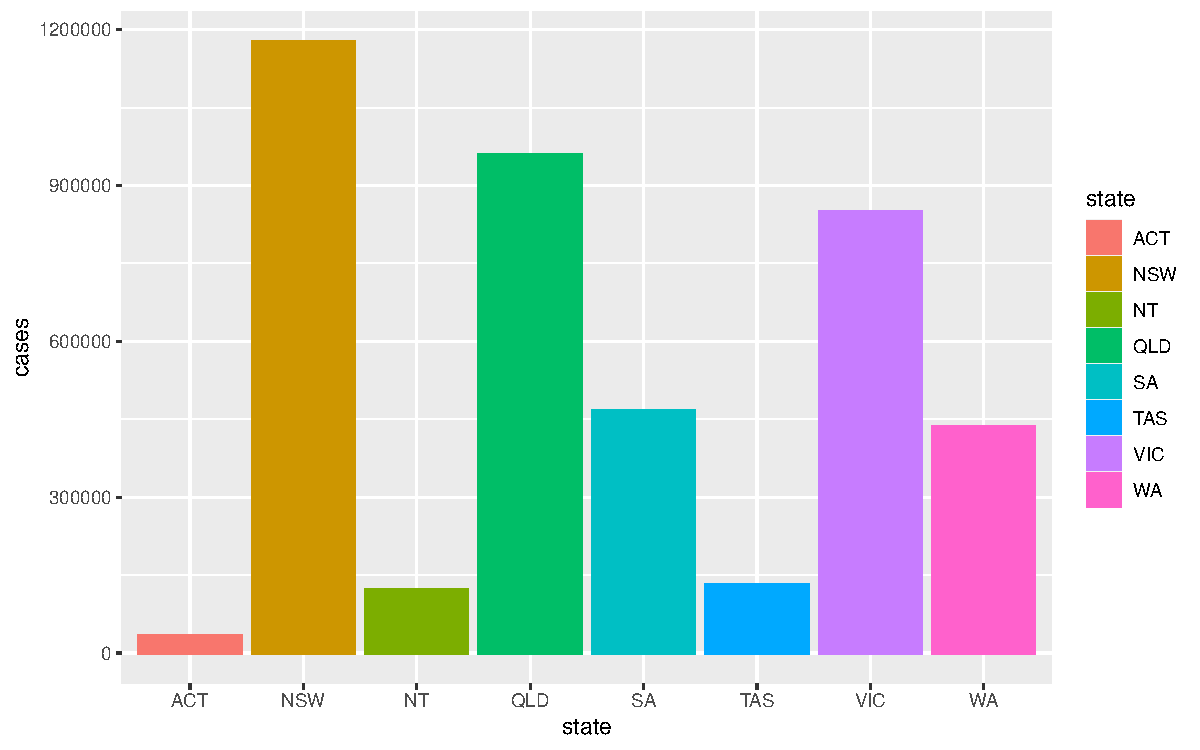
\includegraphics{ETC5513-Assignment4_files/figure-latex/graph1-1.pdf}
\caption{\label{fig:graph1}state-crime}
\end{figure}

The figure above demonstrates high crime cases recorded by NSW, QLD, SA, VIC and WA. However, the high number of crime cases recorded in these states may due to its high population compared to other states/territories like ACT, NT and TAS.

Next, We'd like to look into the frequency of the principal offence in 2018 for top 4 crime-level states. (NSW, QLD, SA and VIC)

\begin{figure}
\centering
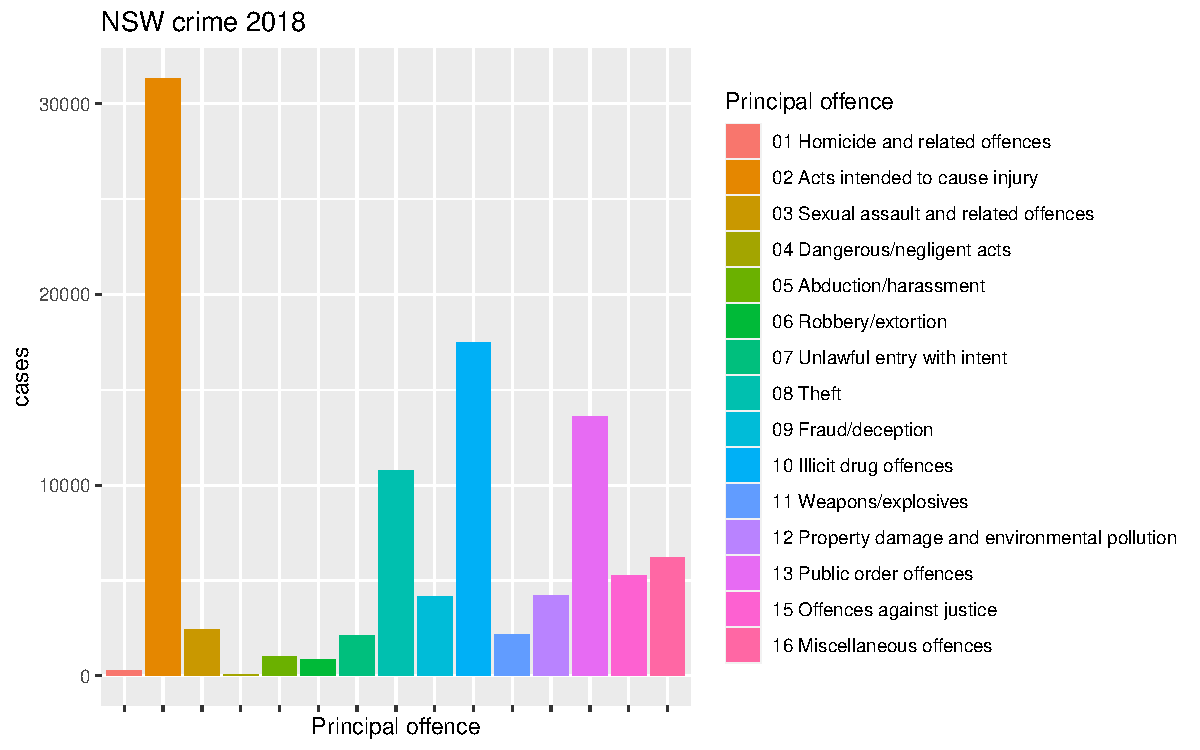
\includegraphics{ETC5513-Assignment4_files/figure-latex/nsw-1.pdf}
\caption{\label{fig:nsw}NSW crime 2018}
\end{figure}

The figure \ref{fig:nsw} demonstrates that 02 Acts intended to cause injury takes the largest proportion in NSW's 2018 crime statistics.

\begin{figure}
\centering
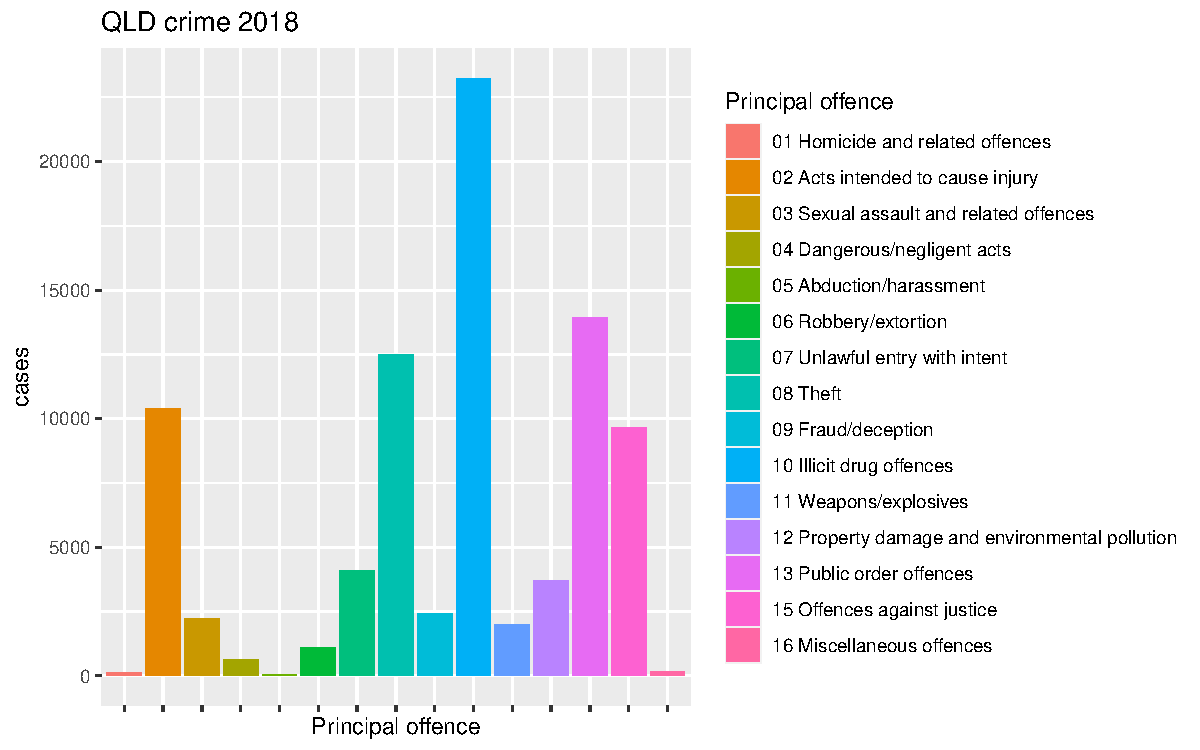
\includegraphics{ETC5513-Assignment4_files/figure-latex/qld-1.pdf}
\caption{\label{fig:qld}QLD crime 2018}
\end{figure}

The figure \ref{fig:qld} demonstrates that 10 Illicit drug offences takes the largest proportion in QLD's 2018 crime statistics. So why some states like QLD have drug offences on rife? Tony Fleming explains in the brisbane times that, ``Largely it is because the Valley and CBD is a night and party precinct. A lot of the drug use is associated with people socialising and whatnot.''\emph{(\textcite{brisbanetimes2019})}

\begin{figure}
\centering
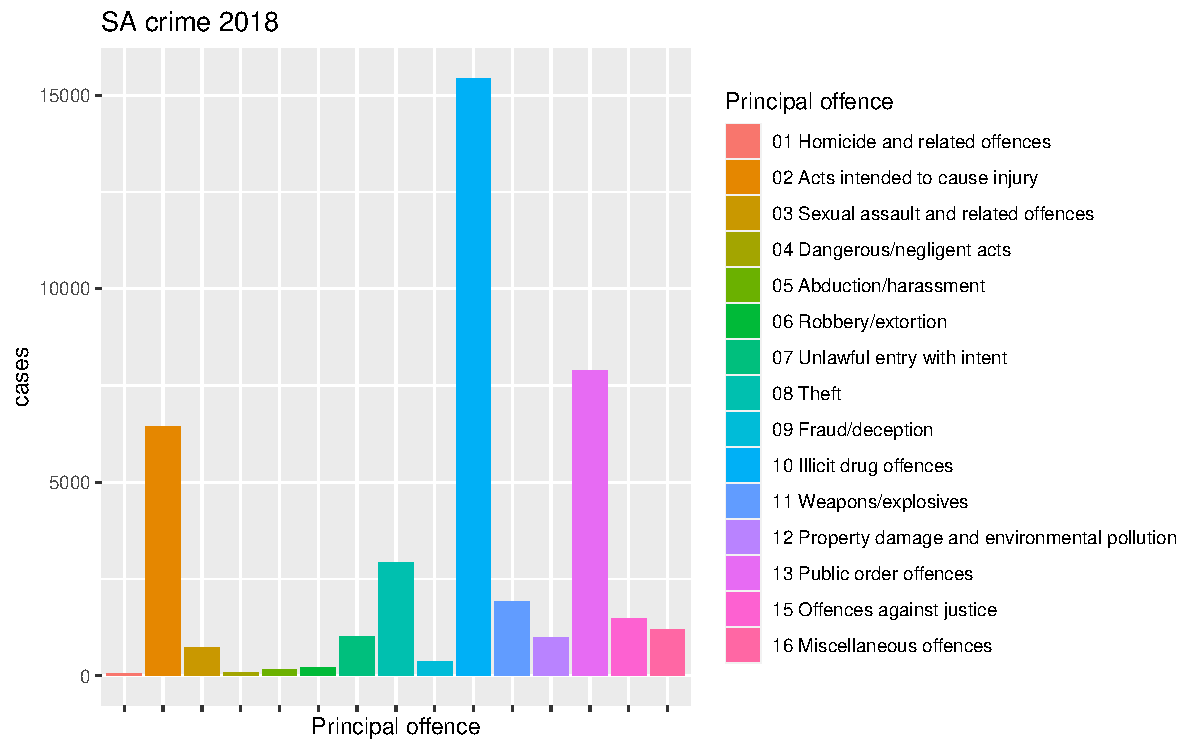
\includegraphics{ETC5513-Assignment4_files/figure-latex/sa-1.pdf}
\caption{\label{fig:sa}SA crime 2018}
\end{figure}

The figure \ref{fig:sa} also represents the outstanding proportion of 10 Illicit drug offences in South Australia's 2018 crime statistics.

\begin{figure}
\centering
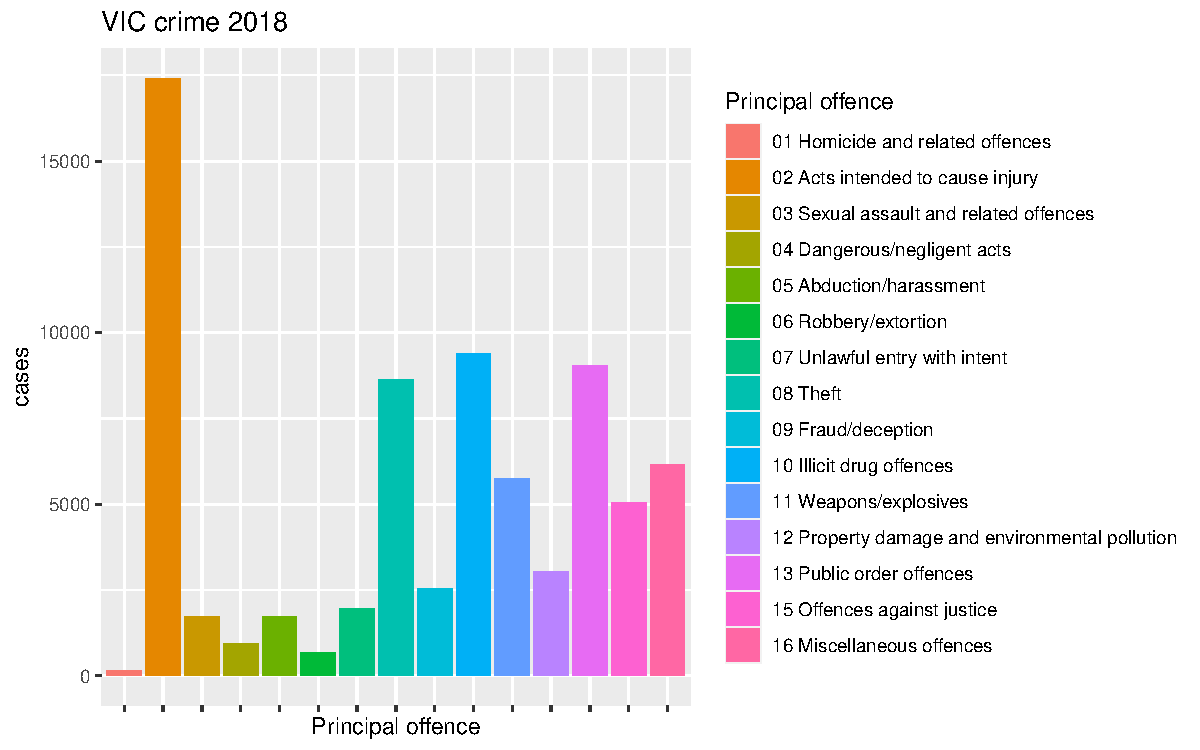
\includegraphics{ETC5513-Assignment4_files/figure-latex/vic-1.pdf}
\caption{\label{fig:vic}VIC crime 2018}
\end{figure}

In the figure \ref{fig:vic}, 02 Acts intended to cause injury resulted in the highest proportion compared to other offences recorded in Victoria's crime statistics.

Furthermore, table \ref{tab:table} also implies the top 4 states accounted for highest proportion of total crime cases recorded in Australia 2018.

\pagebreak

\section*{body 4}

\hypertarget{conclusion}{%
\section{Conclusion}\label{conclusion}}

The crime offender's dataset collected by the Australian Bureau of Statistics allows our group to analyse the insight of the crime circumstances in Australia by gender, age group, states/territories, and police proceedings. The number and rate of male offenders recorded in Australia are significantly higher than that of female offenders. Although the number of offences on both genders has increased in recent years, the growth rate in the number of male offenders is lower than that of females. The rate of male offenders has dropped far more than females. Besides, the majority of the proportion of offenders is from younger age groups. One interesting thing is that the number of offences for the age group below 45 decreased in 2018-2019, while it increased for the age group over 45. Even though the total number of offenders differs across age groups, the trend is pretty similar with 10, 2, 13 being the top three highest principal offences. On the other hand, through the visualisations created for crime statistics on states/territories, the report concludes the top 4 states/territories as NSW, QLD, SA, and VIC. The common grounds of these states are, QLD and SA both had `Illicit drug offences' as the most frequent primary offence, whereas, NSW and VIC had `Acts intended to cause injury'. Lastly, it can be clearly concluded that most criminals will be prosecuted by the court in all states. But offenders in SA and TAS have a smaller proportion of criminals result in court action compared to other states. Most types of crime will result in court actions. However, public order offenses and miscellaneous offenses have less possibility to be litigated by the court.

\hypertarget{acknowledgement}{%
\section{Acknowledgement}\label{acknowledgement}}

The dataset used is offenders dataset of Australia (\textcite{ABS}).
Packages used are \textcite{ggplot2}, \textcite{tidyverse}, \textcite{tinytex}, \textcite{float}, \textcite{lubridate}, \textcite{readxl}, \textcite{kable}, \textcite{bookdown}, \textcite{gridExtra}, \textcite{here}, \textcite{dplyr}, and \textcite{readr}.

\newpage

\printbibliography[title=Reference]

\end{document}

